\documentclass[12pt]{article}
\usepackage[utf8]{inputenc}
\usepackage{polski}
\usepackage[a4paper, left=2.0cm, right=2.0cm, top=2.0cm, bottom=2.0cm]{geometry}
\usepackage{graphicx}
\usepackage{multicol}
\usepackage{hyperref}
\usepackage{skull}
\usepackage[section]{placeins}


\title{PIISW, W04, IO, 2021/2022, semestr letni\\Lista zadań nr 3: Tworzenie i testowanie backendu: serwisy RESTowe}
\author{Marcin Nowak\\ \small marcin.nowak@pwr.edu.pl}

\begin{document}
    \maketitle

    \section*{Zasady oddawania zadań}
    \begin{enumerate}
        \item Rozwiązania zadań muszą być umieszczone w~prywatnym repozytorium na \texttt{git\-hub.com}.
        \item Prowadzący musi mieć uprawnienia do odczytu i~zapisu dla tego repozytorium.
        \item Podczas zajęć konieczne jest pokazanie prowadzącemu skompilowanej i działającej wersji aplikacji.
    \end{enumerate}

    \section*{Wprowadzenie}
    W bardzo popularnej dziś architekturze mikroserwisowej, jednym ze stosowanych wzorców jest Command Query Responsible Segregation (CQRS).
    Umożliwia on oddzielenie części logiki odpowiedzialnej za utrzymanie danych (Create, Update, Delete) od ich odczytu (Read).
    Serwis związany z odczytem może wówczas stosować inny sposób przechowywania danych (joiny nie są efektywne),
    aniżeli relacyjny, który z kolei dobrze odgrywa swoją rolę przy serwisie transakcyjnym (tutaj od utrzymania danych).
    \\
    \begin{figure}[!htb]
        \centering
        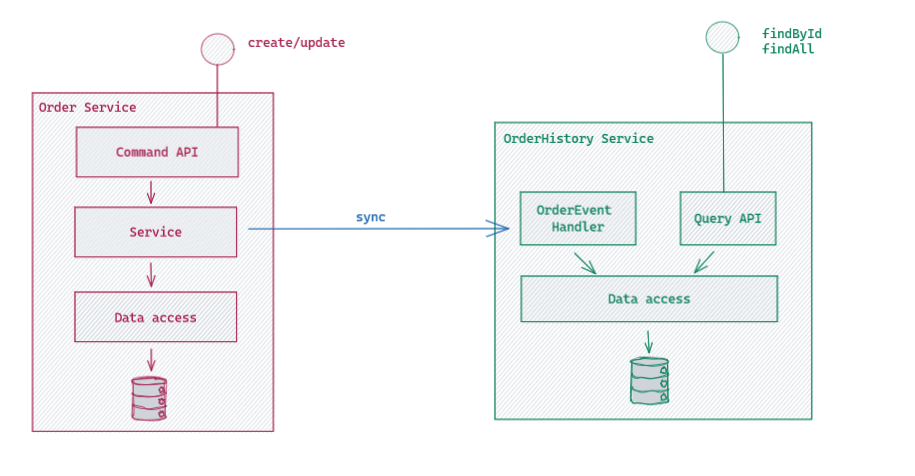
\includegraphics[width=0.75\textwidth]{lista-3-cqrs-diagram.png}
        \caption{Diagram przedstawiający koncepcję Command Query Responsible Segregation}
        \label{fig:cqrs-diagram}
    \end{figure}
    \section*{Oceny}
    \begin{tabular}{|l|c|c|c|c|c|c|c|}
        \hline
        Punkty: & $<9$ & $9-10$ & $11-12$ & $13-14$ & $15-16$ & $17-18$ & $19-20$\\
        \hline
        Ocena: & $2,0$ & $3,0$ & $3,5$ & $4,0$ & $4,5$ & $5,0$ & $5,5$\\
        \hline
    \end{tabular}

    \section*{Zadania}
    \begin{enumerate}
        \item\label{exc:order_service}
            (3 pkt) Order Service

            Utwórz aplikację Order, która spełni następujące kryteria:
            \begin{enumerate}
                \item będzie oparta na \texttt{Spring Boot} (\url{https://start.spring.io}),
                \item zbudowana za pomocą \texttt{Maven},
                \item wykorzysta bazę danych \texttt{H2},
                \item dane z bazy danych będą dostępne pod adresem host:port/h2-console,
                \item wystawi REST API do tworzenia obiektu typu Order,
                \item wystawi REST API do aktualizacji statusu dostawy (Created, PickedUp, Delivered) dla danego Order,
                \item definicja REST będzie możliwa do wyświetlenia z poziomu przeglądarki za pomocą host:port/swagger-ui/index.html,
                \item encja \texttt{Order} powinna zawierać informacje o kliencie, zamówionych produktach oraz dostawie (patrz rysunek~\ref{fig:cud-model}.),
                \item ma odpowiednie pakiety wewnątrz warstwy: REST API, serwisową, dostępu do bazy danych.
            \end{enumerate}

        \item\label{exc:order_history_service}
            (5 pkt) OrderHistory Service.

            Utwórz aplikację OrderHistory, która spełni następujące kryteria:
            \begin{enumerate}
                \item będzie oparta na \texttt{Spring Boot} (\url{https://start.spring.io}),
                \item zbudowana za pomocą \texttt{Maven},
                \item wykorzysta bazę danych \texttt{H2},
                \item dane z bazy danych będą dostępne pod adresem host:port/h2-console,
                \item encja \texttt{OrderHistory} powinna zawierać informacje o kliencie, dostawie oraz zamówionych produktach (nazwy po przecinku w jednym polu) wraz z sumaryczną wartością zamówienia (patrz rysunek~\ref{fig:read-model}.),
                \item ma oddzielone pakiety: REST API, serwisową, dostępu do bazy danych,
                \item wystawi REST API do tworzenia obiektu typu \texttt{OrderHistory} oraz odczytu danych tego typu (GET - na podstawie id oraz wszystkich zapisanych),
                \item definicja REST będzie możliwa do wyświetlenia za pomocą host:port/swagger-ui/index.html,
                \item strona swagger-ui/index.html grupuje operacje (metody do odczytu oddzielnie od tych do tworzenia, patrz ~\ref{fig:swagger-orders-gr} oraz ~\ref{fig:swagger-sync-gr}),
                \item logika zawarta w serwisie jest pokryta testami jednostkowymi (\texttt{JUnit}, \texttt{Mockito}).
            \end{enumerate}

        \item\label{exc:cqrs_sync}
            (3 pkt) Synchronizacja danych pomiędzy Order Service a OrderHistory Service.

            Zarówno po utworzeniu obiektu typu Order jak i zmianie statusu jego dostawy przez Order Service, dane w OrderHistory Service powinny zostać wzbogacone o te zmiany (synchronizacja).
            Do tego celu użyj REST API udostępnionego przez OrderHistory Service.
        \item\label{exc:openapi}
            (4 pkt) Open API.

            Aplikacja OrderHistory Service powinna udostępniać plik Open API (.json lub .yaml), który posłuży Order Service do wygenerowania kodu potrzebnego do połączenia poprzez REST API z OrderHistory Service.

            \textbf{Wskazówka:} Zacznij od wygenerowania pliku z definicją Open API (\url{https://springdoc.org/}). Następnie odpowiednio skorzystaj z mavenowego pluginu: \texttt{openapi-gene\-ra\-tor-ma\-ven-plu\-gin}. Wygenerowany kod powinien znaleść się w katalogu target.
        \item\label{exc:openapi}
        $\skull$(2 pkt) RESTful API i paginacja.

            Rozszerz działanie REST API w OrderHistory Service o metodę wyszukującą zamówienia wraz z możliwością pagingu.

            \textbf{Wskazówka:} Skorzystaj ze Spring HATEOAS.
    \end{enumerate}
    \begin{figure}[p]
        \centering
        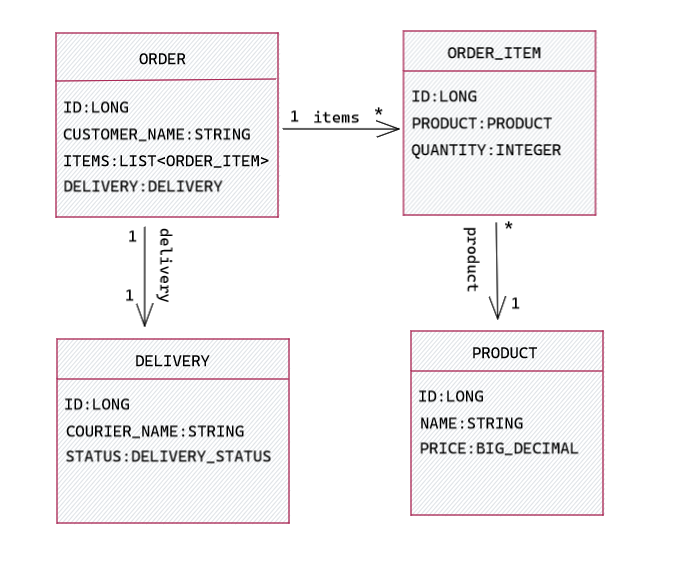
\includegraphics[width=0.9\textwidth]{cud_model.png}
        \caption{Model danych dla zadania~\ref{exc:order_service}.}
        \label{fig:cud-model}
    \end{figure}
    \begin{figure}[p]
        \centering
        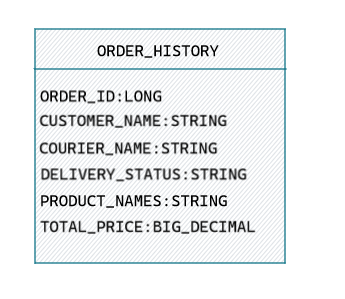
\includegraphics[width=0.5\textwidth]{read-model.png}
        \caption{Model danych dla zadania~\ref{exc:order_history_service}.}
        \label{fig:read-model}
    \end{figure}
    \begin{figure}[p]
        \centering
        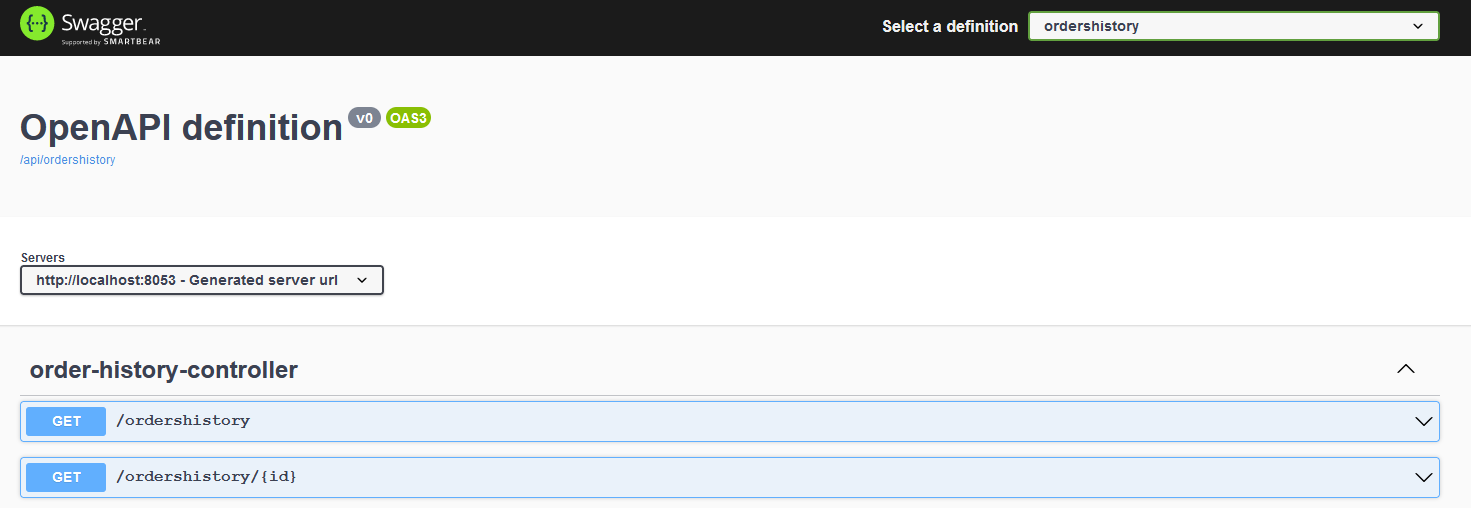
\includegraphics[width=0.8\textwidth]{lista-3-2-a}
        \caption{Przykładowy widok grupy ordershistory na swagger-ui dla zadania~\ref{exc:order_history_service}.}
        \label{fig:swagger-orders-gr}
    \end{figure}
    \begin{figure}[p]
        \centering
        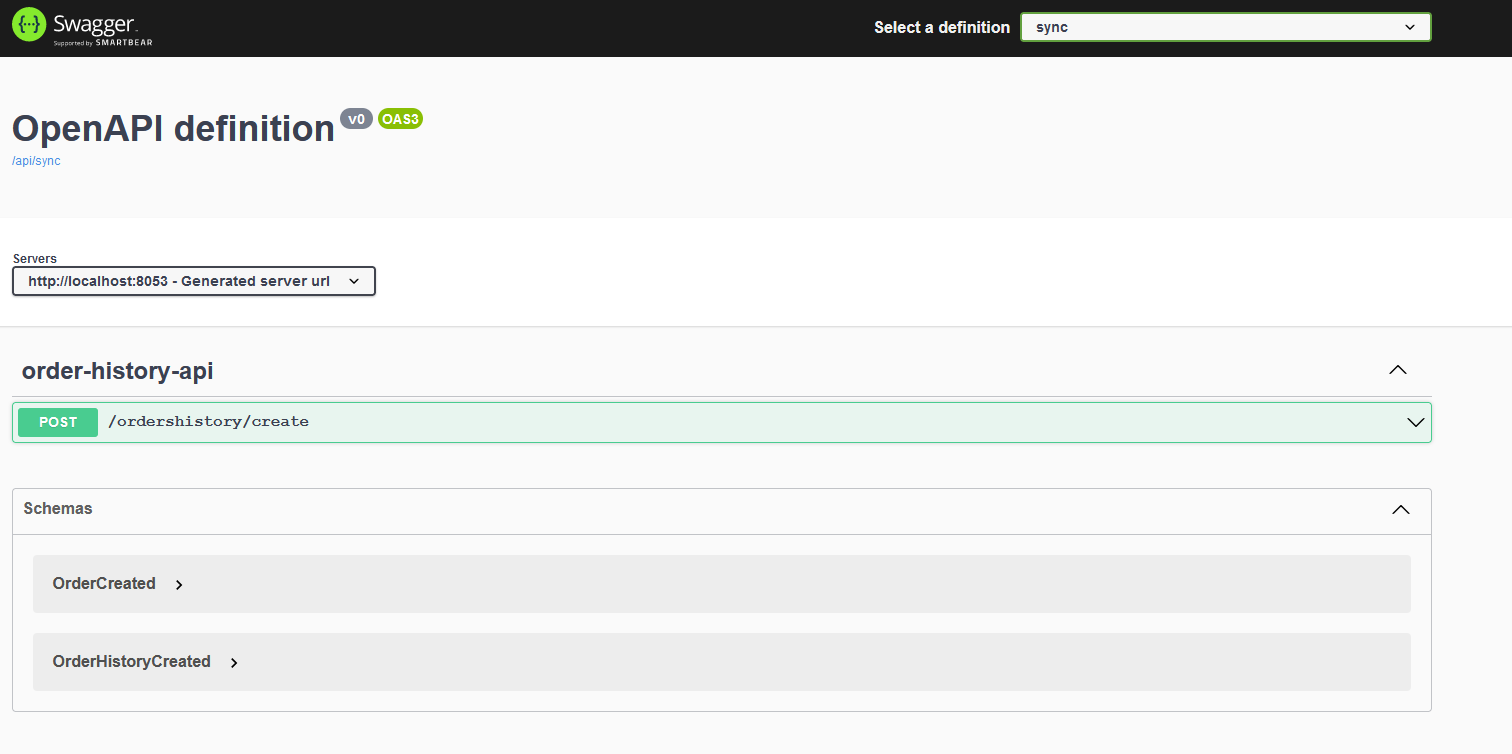
\includegraphics[width=0.8\textwidth]{lista-3-2-b}
        \caption{Przykładowy widok grupy sync na swagger-ui dla zadania~\ref{exc:order_history_service}.}
        \label{fig:swagger-sync-gr}
    \end{figure}
    \begin{figure}[p]
        \centering
        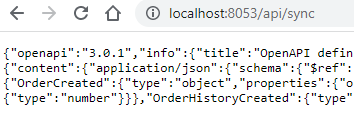
\includegraphics[width=0.6\textwidth]{lista-3-3-a}
        \caption{Przykładowa zawartość pliku Open API do generowania kodu dla zadania~\ref{exc:cqrs_sync}.}
        \label{fig:openapi-gen}
    \end{figure}
\end{document}

